\subsection{API REST}

\begin{frame}{Nos réalisations}{API REST}

\textbf{Les routes de l'application}

\begin{table}
    \begin{tabulary}{\textwidth}{|C C C|}
        \hline
        \rowcolor{primaryLight}\color{background}{Méthode HTTP} & \color{background}{URI} & \color{background}{Paramètres}\\
        \hline
	    GET & api/subnet & \\
	    POST & api/subnet?<parametres> & ip, next\_hop, communities \\
	    PUT & api/subnet?<parametres> & TOUS \\
	    PATCH & api/subnet?<parametres> & id, is\_activated \\
	    DELETE & api/subnet?<parametre> & id \\
	    \hline
	\end{tabulary}
\end{table}
\end{frame}

\begin{frame}{Nos réalisations}{Architecture de l'API REST}
    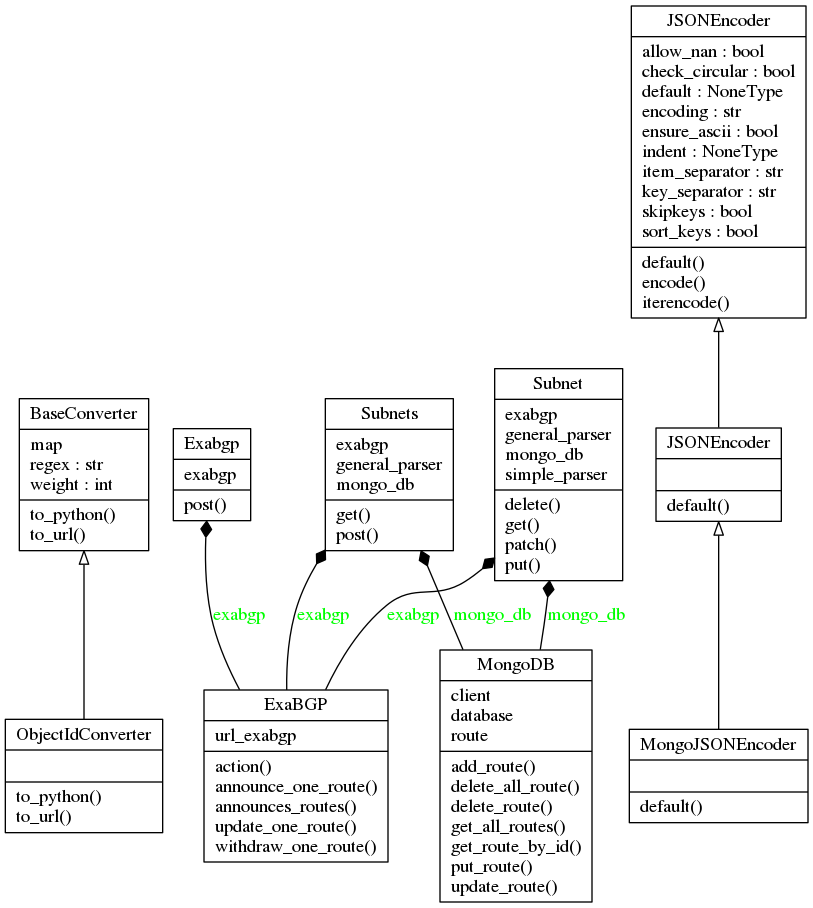
\includegraphics[width=\textwidth, height=0.7\textwidth]{classes_backend.png}
\end{frame}